\section{Heurística golosa}

% Desgraciadamente, el problema es tan difícil que ni Marty ni el Doc conocen
% una manera de resolverlo en tiempo polinomial para el caso general. Para no
% quedarse con las manos vacías, Marty les pide diseñar e implementar una
% heurística constructiva golosa para MCS y desarrollar los siguientes puntos
% para conocer la calidad de las soluciones que le proveerán:
% a) Explicar detalladamente el algoritmo implementado.
% b) Calcular el orden de complejidad temporal de peor caso del algoritmo.
% c) Describir instancias de MCS para las cuales la heurística no proporciona
%    una solución óptima. Indicar qué tan mala puede ser la solución obtenida
%    respecto de la solución óptima.
% d) Realizar una experimentación que permita observar la performance del
%    algoritmo en términos de tiempo de ejecución en función del tamaño de
%    entrada.

\subsection{Introducción}

Dado que la complejidad del algoritmo exacto resulta prohibitiva en la práctica,
se pedía desarrollar una heurística golosa que resolviera el problema en tiempo
polinomial. Para esto fue necesario plantear algoritmos que a cuestas de la
calidad final de la solución permitieran mejorar sustancialmente la complejidad.

Pensar heurísticas tiene el desafío de que las mismas suelen tener un factor
importante de intuición sobre por qué podrían llegar a funcionar mejor o peor y
no una justificación formal. Esto tiene como consecuencia que resulta
difícil decidir qué criterio utilizar puesto que siempre es posible
encontrar instancias para las cuales el mismo sea tan malo como uno
quiera.

El criterio seleccionado fue el grado de los nodos. La motivación detrás de esta
decisión fue la idea de que tomando los vértices de mayor grado en cada grafo,
uno aumenta la posibilidad de que tengan vecinos en común, permitiendo así mapear
sus respectivas aristas en el subgrafo común.

\subsection{Resolución algorítmica}

Se desarrollaron dos algoritmos golosos. El primero trabaja únicamente con la idea de mapear
los nodos de grado mayor de ambos grafos. El segundo toma el algoritmo anterior con
la diferencia de que además de mapear los nodos, agrega el mayor número posible de
vecinos de los mismos. Esta pequeña variación se utilizó como para tener una
alternativa contra la cual comparar. Luego de pruebas que serán discutidas en la
sección de experimentación, se llegó a la conclusión de que esta variación
brindaba peores soluciones que el primer algoritmo, con lo cual todo futuro
análisis será dedicado al primero.

El mecanismo del algoritmo es el siguiente:
\begin{enumerate}
	\item Se utilizan dos colas de prioridad para tener los nodos de cada grafo
	ordenados por mayor grado.
	\item Desencolando el primer nodo de cada cola se forma un par que es agregado al subgrafo común.
	\item Si hay vecinos de los nodos del nuevo par mapeados al mismo elemento del
	subgrafo común, se agrega una arista entre estas asignaciones.
\end{enumerate}

A continuación, el pseudocódigo de la heurística implementada:

\begin{algorithm}[H]
	\SetAlgoVlined
	\caption{Heurística golosa}
	\Input{Dos grafos $G_1$ y $G_2$}
	\Output{Un subgrafo común entre $G_1$ y $G_2$}
	\textit{subgrafo\_común} $\gets$ Crear grafo de pares vacío \;
	\textit{nodos\_sin\_visitar\_g1} $\gets$ Crear cola de prioridad con nodos de $G_1$ utilizando
	su grado como peso \;
	\textit{nodos\_sin\_visitar\_g2} $\gets$ Crear cola de prioridad con nodos de $G_2$ utilizando
	su grado como peso \;

	\textit{vecinos\_mapeados} $\gets$ Crear conjunto de pares vacío \;
	\While{\textit{nodos\_sin\_visitar\_g1} y \textit{nodos\_sin\_visitar\_g2}
	no estén vacíos}{
		\textit{nodo\_g1} $\gets$ Desencolar primero de
		\textit{nodos\_sin\_visitar\_g1} \;
		\textit{nodo\_g2} $\gets$ Desencolar primero de
		\textit{nodos\_sin\_visitar\_g2} \;
		Agregar nodo (\textit{nodo\_g1}, \textit{nodo\_g2}) a
		\textit{subgrafo\_común} \;

		\ForEach{\textit{vecino} de \textit{nodo\_g1}}{
			\If{\textit{vecino} está mapeado en \textit{subgrafo\_común}}{
				Agregar mapeo de \textit{vecino} a \textit{vecinos\_mapeados} \;
			}
		}

		\ForEach{\textit{vecino} de \textit{nodo\_g2}}{
			\If{\textit{vecino} está mapeado en \textit{subgrafo\_común} y el
			mapeo está en \textit{vecinos\_mapeados}}{
				Agregar arista entre (\textit{nodo\_g1}, \textit{nodo\_g1}) y
				mapeo de \textit{vecino} en \textit{subgrafo\_común} \;
			}
		}
		Vaciar \textit{vecinos\_mapeados} \;
	}
	\Return{\textit{subgrafo\_común}}
\end{algorithm}

\subsection{Complejidad}

La complejidad temporal queda en función de la entrada: $G_1 = (V_1, E_1)$ y $G_2 = (V_2,
E_2)$.

Inicializar las dos colas de prioridad tiene un costo $\ord(N_1 \times \log N_1 + N_2
\times \log N_2)$. Esto se debe a que las mismas están implementadas sobre un heap cuyo costo
de inserción es logarítmico sobre la cantidad de elementos en el mismo.

El ciclo principal corre hasta que alguna de las dos colas se vacíe. En el peor caso
ambas colas tienen el mismo tamaño, con lo cual se desencolarían los $N_1 = N_2$
nodos. En cada iteración del ciclo se recorren todos los vecinos de los nodos
desapilados donde para cada uno se realiza una operación de costo constante.
Como estamos asumiendo que se recorren todos los vértices de cada grafo esto
corresponde a la siguiente sumatoria:

\begin{equation*}
	\ord(\sum_{v \in V_1}^{} \deg(v) + \sum_{v \in V_2}^{} \deg(v)) =
	\ord(2 \times M_1 + 2 \times M_2) = \ord(M_1 + M_2)
\end{equation*}

Una vez finalizado el ciclo, se retorna el subgrafo común encontrado, por lo
tanto el costo final del algoritmo es:

\begin{equation*}
	\ord(N_1 \times \log N_1 + N_2 \times \log N_2 + M_1 + M_2)
\end{equation*}

\subsection{Instancias subóptimas}\label{sec:ej4:suboptimal}

Como se dijo anteriormente, una heurística puede funcionar relativamente bien
para algunas instancias y sin embargo ser desastrosa para otras. Para este
problema en particular, las instancias son los pares de grafos ($G_1$, $G_2$) que
son recibidos como entrada.

La heurística golosa desarrollada utiliza fuertemente la intuición de que los
nodos de mayor grado al poseer más vecinos tienen una mayor posibilidad de
agregar aristas contra el subgrafo común generado hasta el momento. Como es de
esperarse, esto puede llevar por mal camino.

Se procede a describir la construcción para una familia de instancias donde el
algoritmo no es capaz de encontrar una arista independientemente del tamaño
de los grafos:

\begin{enumerate}
	\item Crear un ciclo $C_k$ en $G_1$ y $G_2$ con $k \geq 3$.
	\item Crear $k$ estrellas $K_{1,3}$ en $G_1$.
\end{enumerate}

Esto resulta en un grafo $G_1$ con $N_1 = 5 \times k$ y $M_1 = 4 \times k$,
y otro grafo $G_2$ con $N_2 = k$ y $M_2 = k$. Por lo tanto, las instancias
pueden ser tan grandes como uno desee.

El máximo subgrafo común de esta familia siempre será el ciclo $C_k$. Esto se
debe a que $G_2 = C_k$, por lo tanto es subgrafo de $G_1$ que contiene a $C_k$.

El grado máximo de $G_1$ será 3, correspondiente al de los nodos
centrales en cada estrella $K_{1,3}$. En $G_2$ el grado máximo será 2, ya que al
ser un ciclo simple todo vértice tendrá ese número de aristas incidentes.

\begin{figure}[H]
	\centering
	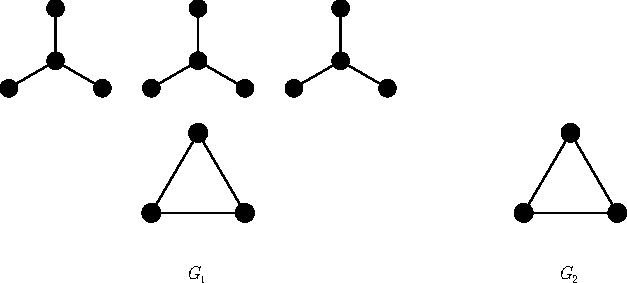
\includegraphics{imagenes/ex4.pdf}
	\caption{Ejemplo de instancia de la familia para $k = 3$.}
	\label{fig:heuristica-golosa:ejemplo-g1-suboptimo}
\end{figure}

Habiendo presentado las características de esta instancia es posible demostrar
que el algoritmo no es capaz de realizar ni un solo mapeo de aristas válido.

Previamente se explicó que la heurística golosa encola todos los nodos de cada
grafo utilizando su grado como prioridad. Esto produce que para $G_1$ estén
primeros todos los nodos centrales de las estrellas $K_{1,3}$ mientras que para
$G_2$ los vértices que componen el ciclo. Al entrar al ciclo principal, se mapea
cada nodo central de alguna estrella de $G_1$ con un vértice perteneciente al
ciclo de $G_2$. Como hay $k$ estrellas y $G_2 = C_k$ cada nodo del ciclo
termina siendo mapeado al vértice central de un $K_{1,3}$.

Este mapeo tiene la particularidad de que no permite agregar ninguna arista, y
esto se debe a que para poder mapear una arista, es necesario que para el par de
nodos a agregar, exista en el subgrafo común un par mapeado con vecinos de ambos
vértices. Cada estrella pertenece a una componente conexa distinta, con lo cual
no hay ninguna arista entre dos estrellas distintas. Como consecuencia, ningún
nodo central de una estrella es vecino a otro. De esta forma, ningún par de
vértices mapeados de $G_1$ es vecino entre sí, produciendo que no sea posible
agregar una arista en el subgrafo común generado.

\begin{figure}[H]
	\centering
	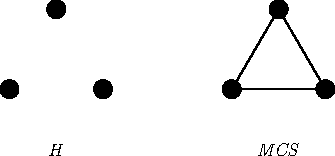
\includegraphics{imagenes/ex4_solution.pdf}
	\caption{$H$ solución generada por la heurística y $MCS$ el máximo subgrafo
	común para la instancia en Figura \ref{fig:heuristica-golosa:ejemplo-g1-suboptimo}.}
	\label{fig:heuristica-golosa:ejemplo-g1-suboptimo-solucion}
\end{figure}

Esto vale para cualquier instancia de esta familia con $k \geq 3$, donde el
algoritmo siempre va a actuar de la misma manera con el peor resultado posible
que es no encontrar ni una arista en común.

\subsection{Experimentación}

La experimentación de este ejercicio estará dividida en dos secciones: una
dedicada a la calidad de soluciones, y otra a la complejidad teórica.

\subsubsection{Calidad de soluciones}

Como se planteó en la introducción, además del algoritmo descrito, se desarrolló
una pequeña variación del mismo para tener un parámetro de comparación adicional
y ver qué tanto podían cambiar las soluciones obtenidas.

La única diferencia que presenta esta alternativa con respecto a la heurística
desarrollada en profundidad, es a la hora de mapear un nodo:

\begin{enumerate}
	\item Toma un nodo de mayor grado de cada grafo.
	\item Agrega este par al subgrafo común junto a todas las aristas que le sea
		posible.
	\item Agrega el mayor número posible de vecinos del par.
	\item Agrega las aristas hacia los vecinos mapeados en el subgrafo común.
\end{enumerate}

La motivación detrás de esta modificación era evitar problemas como el presentado en
la Sección \ref{sec:ej4:suboptimal}, donde por agregar únicamente los vértices de
grado máximo podía suceder que sus vecinos quedaran fuera del mapeo.

Para determinar la calidad de las soluciones se utilizaron los dos conjuntos de
instancias presentados en la introducción del trabajo. De esta forma es posible estudiar
el comportamiento para distintas familias de grafos y para el grupo con
soluciones conocidas incluso analizar qué tan lejos del óptimo estaban los
resultados obtenidos.

Luego de ejecutar las heurísticas golosas sobre las instancias mencionadas, se
generó una tabla para cada grupo con la siguiente información:

\begin{itemize}
	\item Nombre de la instancia.
	\item En caso de conocer la solución, $\#E(MCS)$ el número de aristas de la
		misma.
	\item $\#E(H)$ el número de aristas obtenidos por la heurística base.
	\item $\#E(H_{alt})$ el número de aristas obtenidos por la variación de la heurística base.
	\item $\% \Delta$ la diferencia porcentual entre el número de aristas de $H$
		con respecto a $H_{alt}$.
\end{itemize}

\pgfplotstableread[header=false]{../exp/ej4/known_sol_greedy_exp}{\knowngreedy}
\pgfplotstableread[header=false]{../exp/ej4/unknown_sol_greedy_exp}{\unknowngreedy}

\pgfplotstableread[header=false]{../exp/ej4/known_sol_greedy_add_neighbours_exp}{\knowngreedyaddneighbours}
\pgfplotstableread[header=false]{../exp/ej4/unknown_sol_greedy_add_neighbours_exp}{\unknowngreedyaddneighbours}

\pgfplotstableread[header=false]{../exp/optimal_solutions}{\optimalsolutions}

\pgfplotstablecreatecol
	[copy column from table={\optimalsolutions}{[index] 1}]{sol}{\knowngreedy}
\pgfplotstablecreatecol
	[copy column from table={\knowngreedyaddneighbours}{[index] 1}]{alternative}{\knowngreedy}
\pgfplotstablecreatecol
	[copy column from table={\unknowngreedyaddneighbours}{[index] 1}]{alternative}{\unknowngreedy}

\pgfplotstableset{
	every head row/.style={
		after row=\hline
	},
	columns/0/.style={
		column name=\textsc{Instancia},
		column type={l},
		string replace*={_}{\_},
		string type,
		assign cell content/.code={
			\pgfkeyssetvalue{/pgfplots/table/@cell content}{\texttt{##1}}
		}
	},
	columns/sol/.style={
		column name=$\#E(MCS)$,
		int detect
	},
	columns/1/.style={
		column name=$\#E(H)$,
		int detect
	},
	columns/alternative/.style={
		column name=$\#E(H_{alt})$,
		int detect
	},
	create on use/ratio/.style=
		{create col/expr={(\thisrow{1} * 100)/ \thisrow{alternative} - 100}},
	columns/ratio/.style={
		column name=$\% \Delta$,
		column type={r},
		fixed, precision=2,
		postproc cell content/.append style={
			/pgfplots/table/@cell content/.add={}{\%}
		},
		fonts by sign={}{\color{red}}
	}
}

\begin{figure}[H]
	\centering
	\caption{Grupo de instancias con solución óptima conocida}
	\pgfplotstabletypeset[
		columns={0, sol, 1, alternative, ratio}
	]{\knowngreedy}
\end{figure}

\begin{figure}[H]
	\centering
	\caption{Grupo de instancias con solución desconocida}
	\pgfplotstabletypeset[
		columns={0, 1, alternative, ratio}
	]{\unknowngreedy}
\end{figure}

Lo primero que llama la atención de los valores generados, es el pobre desempeño
de la heurística original para instancias de árboles. Tanto en árboles como para
bosques es superado siempre por la variación del algoritmo. Esto puede verse
como una consecuencia de asignar pares de vértices únicamente en base al grado
de los mismos, ya que en árboles se podría presentar un escenario similar al
planteado con las estrellas. Como los árboles tienen el número justo de aristas
para ser conexos, es menos probable que dos nodos cualesquiera estén conectados
entre si, pudiendo explicar así este tipo de comportamiento donde se agregan
nodos pero los mismos no tienen vecinos que pertenezcan al subgrafo común.

Por otra parte, en el resto de las instancias llegan a haber diferencias
porcentuales positivas órdenes de magnitud mayores que las que funcionaba mejor
la variación. En particular, para grafos donde la densidad de aristas es mayor,
los resultados de la heurística golosa principal presentan soluciones
ampliamente mejores. Nuevamente esto puede explicarse justamente por el hecho de
que al haber más aristas, es mayor la posibilidad de que los nodos a ser
mapeados sean vecinos entre sí. Al comparar grafos completos resulta claro
entonces cómo el algoritmo devuelve la solución óptima, siendo que cada vértice
es vecino al resto.

Dado que la primer heurística golosa planteada resultó mejor en un número mayor
de casos que la variación, y puesto que el único tipo de instancias donde la
alternativa es sustancialmente mejor es la de árboles, se terminó decidiendo
elegir el algoritmo original como generador de soluciones golosas para el resto
de las heurísticas implementadas. El motivo por el cual no se le dio mayor peso
al mal desempeño  sobre las familias de árboles se debe a que teniendo en
consideración que estas soluciones luego son tomadas por un algoritmo de
búsqueda local e incluso posiblemente mejoradas por una metaheurística, un árbol
al tener densidad baja de aristas permite un mejor tiempo de ejecución para
estos algoritmos. En contraposición, familias donde se tiene una densidad alta
de aristas resultan más costosos de mejorar con lo cual es preferible que la
heurística golosa presente mejores soluciones en estos casos.

\subsubsection{Complejidad teórica}

Para ratificar que la complejidad teórica calculada corresponde al
comportamiento del algoritmo en la práctica, se midieron los tiempos de
ejecución con $G_1 = G_2$ para las siguientes familias de grafos:

\begin{itemize}
	\item $T_N$: $N$ nodos sin aristas.
	\item $A_N$: Árboles con $N$ nodos.
	\item $K_N$: Completos con $N$ nodos.
\end{itemize}

El objetivo de esto fue tener un experimento donde se midiera únicamente cuánto
afectaba el número de vértices y otros donde poder observar el efecto de
aumentar la densidad de aristas.

Cada experimento se ejecutó con los siguientes parámetros para cada familia:

\begin{itemize}
	\item $T_N$: $1 \leq N \leq  30000$ tomando 250 muestras con 20 repeticiones cada una.
	\item $A_N$: $1 \leq N \leq  55000$ tomando 100 muestras con 30 repeticiones cada una.
	\item $K_N$: $1 \leq N \leq  1000$ tomando 100 muestras con 30 repeticiones cada una.
\end{itemize}

Dado que la complejidad calculada era:

\begin{equation*}
	\ord(N_1 \times \log N_1 + N_2 \times \log N_2 + M_1 + M_2)
\end{equation*}

Tomando $G_1 = G_2$ (puesto que interesa estudiar el peor escenario que es
cuando se recorren ambos grafos por completo) la complejidad se medirá en función
de $N = N_1 = N_2$, $M = M_1 = M_2$ quedando por lo tanto:

\begin{equation*}
	\ord(N \times \log N + M)
\end{equation*}

~

Para la prueba con grafos sin aristas se debería obtener algo del orden $\ord(N
\times \log N)$. Parte del interés en este tipo de instancias es afirmar que al
eliminar las aristas únicamente influyen los costos asociados al número de
vértices en la entrada.

\renewcommand\constante{65}

\begin{figure}[H]
	\centering
	\caption{Tiempo de ejecución con $N = N_1 = N_2$ $(c = \constante)$}
	\begin{tikzpicture}
		\begin{axis}[
				title={},
				xlabel={Tamaño de entrada $N$},
				ylabel={Tiempo de ejecución (nanosegundos)},
				scaled x ticks=false,
				scaled y ticks=false,
				max space between ticks=37,
				enlargelimits=0.05,
				width=0.5\textwidth,
				height=0.5\textwidth,
				legend pos=north west,
				legend cell align=left
			]
			\addplot[color=black]
				table[x index=0, y expr={\constante*x*ln(x)}]{../exp/ej4/add_nodes_exp};
			\addplot[color=red]
				table[x index=0, y index=1]{../exp/ej4/add_nodes_exp};
			\legend{$c \times N \times \log (N)$, $T_N$}
		\end{axis}
	\end{tikzpicture}
	\label{fig:heuristica-golosa:grafos-sin-aristas}
\end{figure}

En la Figura \ref{fig:heuristica-golosa:grafos-sin-aristas} es posible ver cómo
efectivamente el tiempo de ejecución para esta familia de grafos resulta
acotable por una función que corresponde a la complejidad esperada.

\begin{figure}[H]
	\centering
	\captionsetup{justification=centering, width=.7\linewidth}
	\caption{Cociente entre tiempo de ejecución y complejidad teórica para
	entrada $N = N_1 = N_2$ $(c = \constante)$}
	\begin{tikzpicture}
		\begin{axis}[
				title={},
				xlabel={Tamaño de entrada $N$},
				ylabel={Tiempo de ejecución (nanosegundos) / $(N \times \log (N))$},
				scaled x ticks=false,
				scaled y ticks=false,
				max space between ticks=37,
				enlargelimits=0.05,
				width=0.5\textwidth,
				height=0.5\textwidth,
				legend pos=north west,
				legend cell align=left,
				restrict x to domain=200:30000,
				ymax=200
			]
			\addplot[color=black]
				table[x index=0, y expr={\constante}]{../exp/ej4/add_nodes_exp};
			\addplot[color=red]
				table[x index=0, y expr={\thisrowno{1}/(x*ln(x))}]{../exp/ej4/add_nodes_exp};
			\legend{$c$, $T_N / (N \times \log (N))$}
		\end{axis}
	\end{tikzpicture}
	\label{fig:heuristica-golosa:grafos-sin-aristas-cociente}
\end{figure}

En la Figura \ref{fig:heuristica-golosa:grafos-sin-aristas-cociente} se confirma
lo comentado al poder mostrar que al dividir los tiempos de ejecución se obtiene
una gráfico que converge hacia una constante.

~

Para la familia $A_N$ se deseaba estudiar cómo afecta la densidad de aristas. En
particular dado que estas instancias corresponden a árboles se tiene $M = N -
1$, por lo tanto la complejidad resultante quedaría en el orden de
$\ord(N \times \log N + N)$.

\renewcommand\constante{150}

\begin{figure}[H]
	\centering
	\caption{Tiempo de ejecución con árboles de tamaño $N = N_1 = N_2$ $(c = \constante)$}
	\begin{tikzpicture}
		\begin{axis}[
				title={},
				xlabel={Tamaño de entrada $N$},
				ylabel={Tiempo de ejecución (nanosegundos)},
				scaled x ticks=false,
				scaled y ticks=false,
				enlargelimits=0.05,
				width=0.5\textwidth,
				height=0.5\textwidth,
				legend pos=north west,
				legend cell align=left
			]
			\addplot[color=black]
				table[x index=0, y expr={\constante*(x*ln(x) + x)}]{../exp/ej4/add_tree_nodes_exp};
			\addplot[color=red]
				table[x index=0, y index=1]{../exp/ej4/add_tree_nodes_exp};
			\legend{$c \times (N \times \log (N) + N)$, $A_N$}
		\end{axis}
	\end{tikzpicture}
	\label{fig:heuristica-golosa:arboles}
\end{figure}

Es posible ver en Figura \ref{fig:heuristica-golosa:arboles} como el
tiempo de ejecución puede ser acotado por lo estimado anteriormente. Cabe destacar que
para este caso en particular, el costo que agregan las aristas es absorbido por
lo que toma encolar todos los nodos en las colas de prioridad, que tiene un
orden $\ord(N \times \log N)$.

\begin{figure}[H]
	\centering
	\captionsetup{justification=centering, width=.7\linewidth}
	\caption{Cociente entre tiempo de ejecución y complejidad teórica para
	árboles de tamaño $N = N_1 = N_2$ $(c = \constante)$}
	\begin{tikzpicture}
		\begin{axis}[
				title={},
				xlabel={Tamaño de entrada $N$},
				ylabel={Tiempo de ejecución (nanosegundos) / $(N \times \log (N) + N)$},
				scaled x ticks=false,
				scaled y ticks=false,
				enlargelimits=0.05,
				width=0.5\textwidth,
				height=0.5\textwidth,
				legend pos=north west,
				legend cell align=left,
				restrict x to domain=200:55000,
				ymax=400
			]
			\addplot[color=black]
				table[x index=0, y expr={\constante}]{../exp/ej4/add_tree_nodes_exp};
			\addplot[color=red]
				table[x index=0, y expr={\thisrowno{1}/(x*ln(x) + x)}]{../exp/ej4/add_tree_nodes_exp};
			\legend{$c$, $A_N / (N \times \log (N) + N)$}
		\end{axis}
	\end{tikzpicture}
	\label{fig:heuristica-golosa:arboles-cociente}
\end{figure}

Al realizar el cociente, en Figura \ref{fig:heuristica-golosa:arboles-cociente}
se obtiene de nuevo la convergencia hacia un valor constante asegurando así que
el crecimiento de la función fue el proyectado.

~

Finalmente, se presentan los tiempos obtenidos para la familia de completos
$K_N$. En este caso la cantidad de aristas corresponde a $M = \frac{N \times (N -
1)}{2}$. Contrario al caso de los árboles, el número de aristas está en el
máximo posible permitiendo analizar así cómo funciona la heurística golosa
cuando este parámetro es llevado al límite.

Con esta cantidad de aristas, la complejidad resulta en el orden de:

\begin{equation*}
	\ord(N \times \log (N) + \frac{N \times (N - 1)}{2}) =
	\ord(N \times \log (N) + N^2) = \ord(N^2)
\end{equation*}

\begin{figure}[H]
	\centering
	\caption{Tiempo de ejecución con completos de tamaño $N = N_1 = N_2$ $(c = \constante)$}
	\begin{tikzpicture}
		\begin{axis}[
				title={},
				xlabel={Tamaño de entrada $N$},
				ylabel={Tiempo de ejecución (nanosegundos)},
				scaled x ticks=false,
				scaled y ticks=false,
				enlargelimits=0.05,
				width=0.5\textwidth,
				height=0.5\textwidth,
				legend pos=north west,
				legend cell align=left
			]
			\addplot[color=black]
				table[x index=0, y expr={\constante*(x*ln(x) + x*x)}]{../exp/ej4/add_complete_nodes_exp};
			\addplot[color=red]
				table[x index=0, y index=1]{../exp/ej4/add_complete_nodes_exp};
			\legend{$c \times (N \times \log (N) + N^2)$, $K_N$}
		\end{axis}
	\end{tikzpicture}
	\label{fig:heuristica-golosa:completos}
\end{figure}

Ahora sí, en la Figura \ref{fig:heuristica-golosa:completos} no solo se puede
apreciar que los resultados están acotados por el orden de complejidad estimado
si no que para estas instancias ahora es el costo de creación de las colas de
prioridad el que queda absorbido por el procesamiento de las aristas que resulta
cuadrático.

\begin{figure}[H]
	\centering
	\captionsetup{justification=centering, width=.7\linewidth}
	\caption{Cociente entre tiempo de ejecución y complejidad teórica para
	completos de tamaño $N = N_1 = N_2$ $(c = \constante)$}
	\begin{tikzpicture}
		\begin{axis}[
				title={},
				xlabel={Tamaño de entrada $N$},
				ylabel={Tiempo de ejecución (nanosegundos) / $(N \times \log (N) + N^2)$},
				scaled x ticks=false,
				scaled y ticks=false,
				enlargelimits=0.05,
				width=0.5\textwidth,
				height=0.5\textwidth,
				legend pos=north west,
				legend cell align=left,
				restrict x to domain=100:1000,
				ymax=300
			]
			\addplot[color=black]
				table[x index=0, y expr={\constante}]{../exp/ej4/add_complete_nodes_exp};
			\addplot[color=red]
				table[x index=0, y expr={\thisrowno{1}/(x*ln(x) + x*x)}]{../exp/ej4/add_complete_nodes_exp};
			\legend{$c$, $K_N / (N \times \log (N) + N^2)$}
		\end{axis}
	\end{tikzpicture}
	\label{fig:heuristica-golosa:completos-cociente}
\end{figure}

Por última vez, en Figura \ref{fig:heuristica-golosa:completos-cociente} se corroboran
las cotas determinadas al verificar que el cociente lleva a que el resultado
final converja a una constante.

\subsubsection{Conclusiones}

De esta experimentación se puede concluir que el algoritmo respeta la
complejidad teórica calculada previamente. Además, queda en evidencia el peso que tiene la
proporción de aristas, donde se pudo estudiar cómo la complejidad en función de
$N$ varía entre $\ord(N \times \log N)$ y $\ord(N^2)$.
